%  ========================================================================
%  Copyright (c) 1985 The University of Washington
%
%  Licensed under the Apache License, Version 2.0 (the "License");
%  you may not use this file except in compliance with the License.
%  You may obtain a copy of the License at
%
%      http://www.apache.org/licenses/LICENSE-2.0
%
%  Unless required by applicable law or agreed to in writing, software
%  distributed under the License is distributed on an "AS IS" BASIS,
%  WITHOUT WARRANTIES OR CONDITIONS OF ANY KIND, either express or implied.
%  See the License for the specific language governing permissions and
%  limitations under the License.
%  ========================================================================
%

% Documentation for University of Washington thesis LaTeX document class
% by Jim Fox
% fox@washington.edu
%
%    Revised 2020/02/24, added \caption()[]{} option.  No ToC.
%
%    Revised for version 2015/03/03 of uwthesis.cls
%    Revised, 2016/11/22, for cleanup of sample copyright and title pages
%
%    This document is contained in a single file ONLY because
%    I wanted to be able to distribute it easily.  A real thesis ought
%    to be contained on many files (e.g., one for each chapter, at least).
%
%    To help you identify the files and sections in this large file
%    I use the string '==========' to identify new files.
%
%    To help you ignore the unusual things I do with this sample document
%    I try to use the notation
%       
%    % --- sample stuff only -----
%    special stuff for my document, but you don't need it in your thesis
%    % --- end-of-sample-stuff ---


%    Printed in twoside style now that that's allowed
%
 
\documentclass [11pt, proquest] {uwthesis}[2020/02/24]
 
%
% The following line would print the thesis in a postscript font 

% \usepackage{natbib}
% \def\bibpreamble{\protect\addcontentsline{toc}{chapter}{Bibliography}}

\setcounter{tocdepth}{1}  % Print the chapter and sections to the toc
 

% ==========   Local defs and mods
%

% --- sample stuff only -----
% These format the sample code in this document

\usepackage{alltt}  % 
\usepackage[version=4]{mhchem}
\usepackage{xcolor}
\usepackage{graphicx}
\usepackage{booktabs}

\usepackage{epstopdf}
\epstopdfDeclareGraphicsRule{.tif}{png}{.png}{convert #1 \OutputFile}
\AppendGraphicsExtensions{.tif}

\usepackage[backend=biber,style=chem-acs]{biblatex} % use autocite
\newenvironment{demo}
  {\begin{alltt}\leftskip3em
     \def\\{\ttfamily\char`\\}%
     \def\{{\ttfamily\char`\{}%
     \def\}{\ttfamily\char`\}}}
  {\end{alltt}}
 
% metafont font.  If logo not available, use the second form
%
% \font\mffont=logosl10 scaled\magstep1
\let\mffont=\sf
% --- end-of-sample-stuff ---
 
\addbibresource{all_references.bib}

\begin{document}
 
% ==========   Preliminary pages
%
% ( revised 2012 for electronic submission )
%

\prelimpages
 
%
% ----- copyright and title pages
%
\Title{Uses of the Many-Body Expansion for Studying Molecular Interactions and Driving Molecular Dynamics}
\Author{Joseph P. Heindel}
\Year{2022}
\Program{Department of Chemistry}

\Chair{Dr. Sotiris S. Xantheas}{}{}
\Signature{Dr. Anne B. McCoy}
\Signature{Dr. Charles T. Campbell}
\Signature{Dr. Stephanie Valleau}

\copyrightpage

\titlepage  

 
%
% ----- signature and quoteslip are gone
%

%
% ----- abstract
%


\setcounter{page}{-1}
\abstract{
\par The many-body expansion (MBE) is a method of decomposing any molecular property into contributions from the sub-systems of some total system. We focus on applying the MBE to detailed studies of the energy and forces of molecular clusters. In particular, we carry out the MBE up to full order for \ce{(H2O)7} and \ce{(H2O)_{10}} with increasingly complete basis sets. In doing this, we determine that the convergence of higher-order terms in the MBE depends sensitively on the presence of basis set superposition error (BSSE). Namely, the MBE for 3-body and higher terms in the energy is converged with an aug-cc-pVDZ basis set as long as a BSSE correction is included. If BSSE is ignored, however, the MBE oscillates from term to term and converges very slowly.

\par We carry out a similar analysis of ion-water clusters, \ce{Z^{+/-}(H2O)_{9}}, where \ce{Z^{+/-}}= \ce{Li+}, \ce{Na+}, \ce{K+}, \ce{Rb+}, \ce{Cs+}, \ce{F-}, \ce{Cl-}, \ce{Br-}, and \ce{I-}. We verify the same conclusions about convergence of the MBE as for pure water clusters. Additionally, we find a remarkable linear anti-correlation between the total 2-body ion-water and 2-body and 3-body water-water interactions. This provides a quantitative measure of the extent to which hydrogen bond networks are disrupted by the presence of monoatomic ions. For both neutral and ion-water clusters, we find that the correlation energy makes less than 0.1\% total contribution to the energy at the 3-body and higher levels. That is, electron correlation only needs to be included at the 1- and 2-body levels to capture 99.9\% of the energy.

\par These detailed analyses lay the groundwork for a scheme in which high levels of electronic structure theory, such as MP2 and CCSD(T), can be used to drive the molecular dynamics of medium-sized systems without a major loss of accuracy. We first demonstrate that one can use the MBE to drive dynamics simulations with the MB-Pol water potential. These simulations result in the observation that the MBE is very slow to converge the angle between the full forces and forces calculated with the MBE. That is, the norm of the force vector converges at the 3-body level, but the angle between the full force vector and an approximate force vector is converged somewhere between the 4- and 6-body levels depending on how tight of convergence requirements one may have.

\par \textbf{STUFF ABOUT THE AIMD MBE-MD}
}
 
%
% ----- contents & etc.
%
\tableofcontents
\listoffigures
%\listoftables  % I have no tables
 
%
% ----- glossary 
%
\chapter*{Glossary}      % starred form omits the `chapter x'
\addcontentsline{toc}{chapter}{Glossary}
\thispagestyle{plain}
%
\begin{glossary}
\item[argument] replacement text which customizes a \LaTeX\ macro for
each particular usage.
\item[back-up] a copy of a file to be used when catastrophe strikes
the original.  People who make no back-ups deserve
no sympathy.
\item[control sequence] the normal form of a command to \LaTeX.
\item[delimiter] something, often a character, that indicates
the beginning and ending of an argument.
More generally, a delimiter is a field separator.
\item[document class] a file of macros that tailors \LaTeX\ for
a particular document.  The macros described by this thesis
constitute a document class.
\item[document option] a macro or file of macros
that further modifies \LaTeX\ for
a particular document.  The option {\tt[chapternotes]}
constitutes a document option.
\item[figure] illustrated material, including graphs,
diagrams, drawings and photographs.
\item[font] a character set (the alphabet plus digits
and special symbols) of a particular size and style.  A couple of fonts
used in this thesis are twelve point roman and {\sl twelve point roman
slanted}.
\item[footnote] a note placed at the bottom of a page, end of a chapter,
or end of a thesis that comments on or cites a reference
for a designated part of the text.
\item[formatter] (as opposed to a word-processor) arranges printed
material according to instructions embedded in the text.
A word-processor, on the other hand, is normally controlled
by keyboard strokes that move text about on a display.
\item[\LaTeX] simply the ultimate in computerized typesetting.
\item[macro]  a complex control sequence composed of 
other control sequences.
\item[pica] an archaic unit of length.  One pica is twelve points and
six picas is about an inch.
\item[point] a unit of length.  72.27 points equals one inch.
\item[roman]  a conventional printing typestyle using serifs.
the decorations on the ends of letter strokes.
This thesis is set in roman type.
\item[rule] a straight printed line; e.g., \hrulefill.
\item[serif] the decoration at the ends of letter strokes.
\item[table] information placed in a columnar arrangement.
\item[thesis] either a master's thesis or a doctoral dissertation.
This document also refers to itself as a thesis, although it
really is not one.
 
\end{glossary}
 
%
% ----- acknowledgments
%
\acknowledgments{% \vskip2pc
  % {\narrower\noindent
  I wish to thank my wife, Leah Heindel, for showing me what it means to care deeply for others, for showing me how to balance passion with stability, and for always pushing me in better directions than the ones I choose for myself.
  
  Thank you to Daniel Schofield for introducing me to computational chemistry. You prepared me excellently for graduate school. Perhaps more importantly, you showed me that humility and scientific excellence are not mutually exclusive.
  
  Thank you to Anne McCoy for letting me hang around her group. I learned many things about science and being a scientist that I would not have figured out otherwise. You were also excellent at keeping my ego in check, which, on its own, is uncontrollably self-inflating.
  
  Finally, thank you to my advisor, Sotiris Xantheas. You have often treated me like family and I appreciate that immensely. You have given me every opportunity to succeed in science, so I hope I can make something of these favorable initial conditions.
  % \par}
}

%
% ----- dedication
%
\dedication{\begin{center}Who to dedicate this to? 

Perhaps Silicon, without which computational chemistry would be much harder.\end{center}}

%
% end of the preliminary pages
 
 
 
%
% ==========      Text pages
%

\textpages
 
% ========== Chapter 1
 
\chapter {Introduction}
 
The utility of a clean, professionally prepared thesis is well
documented%
\footnote{See, for example,
  W.~Shakespeare\cite{Hamlet} for a recent discussion.}
and, even if you never intend to actually print your thesis,
you still ought to format it as if that were your intention.
 
\TeX\ facilitates that. It is a flexible,
complete and professional typesetting system.
It will produce {\bf pdf} output as required by the Graduate School.

\section{The Purpose of This Sample Thesis}
 
This sample is both a demonstration of the quality and
propriety of a \LaTeX formatted thesis and  
documentation for its preparation.
It has made extensive use of a custom class file
developed specifically for this purpose
at the University of Washington.  Chapter~II discusses
\TeX\ and \LaTeX.
Chapter III describes the additional macros and functions
provided by the custom thesis class file.  Finally, Chapter IV hopes to tie things up.
 
It is 
impossible to predict all the formatting problems one will encounter
and there will be problems that are best handled
by a specialist.  
The Graduate School may be able to help you find help.
Some departments may also be able to provide \LaTeX\ assistance.
 
 
\section{Conventions and Notations}
 
In this thesis the typist
refers to the user of \LaTeX---the one who
makes formatting decisions and chooses the appropriate
formatting commands.
He or she will most often be the degree candidate.
 
This document deals with \LaTeX\ typesetting commands and their
functions.  Wherever possible the conventions used to display
text entered by the typist and the resulting formatted output
are the same as those used by the \TeX books.
Therefore, {\tt typewriter type} is used to indicate text
as typed by the computer
or entered by the typist.
It is quite the opposite of {\it italics,} which indicates
a category rather than exact text.  For example,
{\tt alpha} and {\tt beta} might each be an example of a {\it label}.
 
 
\section{Nota bene}
 
This sample thesis was produced by the \LaTeX\ document class it describes
and its format is consonant with the Graduate School's electronic dissertation guidelines,
as of November, 2014, at least.
However, use of this package does not guarantee acceptability
of a particular thesis.
 
 % ========== BSSE MBE of Water Clusters
 
\chapter{The many-body expansion for aqueous systems revisited: I. Water-water interactions}

\section{Introduction}

\par The Many-Body Expansion (MBE) of the interaction energy of a system of n-fragments is a concept that has its origins in combinatorial mathematics and in particular the inclusion-exclusion principle, a counting technique introduced in the 1700s to obtain the number of elements in the union of finite sets.\autocite{roberts_applied_2009} It was first applied to water in 1970 by Hankins, Moskowitz, and Stillinger\autocite{hankins_water_1970} to obtain the 3-body contribution to the Hartree-Fock (HF) energy of a water trimer configuration consisting of a double donor, a double acceptor and a sequential water (but not to the trimer global ring minimum, which was missed in that study). We have subsequently used it in 1994 to decompose the energies of the minimum energy configurations of ring water clusters dimer through hexamer obtained at the second order Møller-Plesset (MP2) level of theory.\autocite{xantheas_ab_1994} That study also considered the effect of the Basis Set Superposition Error (BSSE) corrections\autocite{boys_calculation_1970, xantheas_importance_1996} to the individual many-body terms of these first few water clusters. A subsequent probe of the magnitudes of these terms for water clusters resembling bulk water configurations suggested that terms higher than two-body are less significant for configurations resembling bulk water, which have on the average two hydrogen bonds per water molecule.\autocite{xantheas_significance_1996} Finally, this analysis was reported for several low-lying minima of the first few water clusters in order to examine the variation of the magnitude of the many-body terms for different hydrogen bonding networks in order to investigate the origin of their relative stabilities.\autocite{xantheas_cooperativity_2000}
\par The interest in the many-body decomposition and in particular questions related to whether the magnitudes of the various terms exhibit a monotonic behavior, or the series converges and at which rank, stems from the need to understand and quantify the cooperative, non-additive (beyond two-body) interactions in water. The non-additive effects result in the shortening of the intermolecular O-O separation in the first few water ring cluster minima\autocite{xantheas_ab_1993, miliordos_optimal_2013} and the lengthening of the intermolecular O-H participating in the hydrogen bonds that causes a red shift in the positions of the corresponding OH vibrations with respect to those in the isolated gas phase monomer.\autocite{burnham_formation_2002} The general consensus that the series practically converges at the three-body term has fueled the development of a new generation of many-body interaction potentials for water such as the family of the Thole-type Models (TTM)\autocite{burnham_parametrization_1999, burnham_development_2002, burnham_development_2002-1, fanourgakis_flexible_2006, fanourgakis_development_2008} subsequent extensions and enhancements implemented in the Huang, Braams, Bowman (HBB2)\autocite{shank_accurate_2009, wang_towards_2010} and the Many-Body polarizable (MB-pol)\autocite{babin_toward_2012, babin_development_2013, babin_development_2013-1, babin_development_2014} models. These approaches are based on fitting separately the 1-, 2-, and 3-body potential energy surfaces (PESs) as well as the 1- and 2-body dipole moment surfaces (DMSs). The families of these potentials have demonstrated unprecedented accuracy for water\autocite{babin_development_2013, babin_development_2014, paesani_quantum_2007} and more recently for hydronium-water complexes\autocite{heindel_benchmark_2018}.
\par In recent years, the many-body expansion (MBE) has become a favorite tool for the accurate description of the molecular properties of water and molecules solvated in water. The MBE has provided an increasingly detailed understanding of the many-body convergence of properties of water ranging from the energies\autocite{xantheas_ab_1994, pedulla_theoretical_1998}, dipole moment and polarizability\autocite{medders_many-body_2013}, local and normal mode vibrational frequencies\autocite{heindel_origin_2018, howard_n-body_2013}, and forces\autocite{bates_efficient_2011, demerdash_convergence_2016, demerdash_assessing_2017}. Furthermore, the use of the MBE offers the possibility of employing highly accurate and computationally expensive \textit{ab initio} methods, such as Coupled Cluster with Singles, Doubles and perturbative estimate of Triples replacements [CCSD(T)] for the fragments of a molecular system, which is typically too large to be described at this level of theory. This, however, comes with the caveat that the number of sub-systems, for which calculations must be carried out, increases combinatorially with each term included in the MBE. Thus, as the system becomes large, it is not clear that using the MBE provides any real time savings unless the MBE is truncated at low-order. This is why it is important to understand when a sub-cluster can be neglected based on some distance or connectivity criteria.\autocite{cui_theoretical_2006, ouyang_when_2016} The MBE can also be used to decompose very large molecules, such as proteins, into subunits for smaller calculations.\autocite{mayhall_many-overlapping-body_2012, richard_many-body_2013} This scheme does provide a speedup relative to the full calculation, however these schemes typically involve splitting a system along a covalent bond, so the results can vary according to which subunits are chosen to reconstruct the whole system. Their flexibility exists in how these subunits are chosen, such as in the fragmentation of overlapping-bodies or in other fragmentation schemes of molecular clusters. These schemes have been unified in the so-called generalized MBE.\autocite{richard_generalized_2012}

\par There still exist outstanding questions regarding the convergence of the MBE for larger systems in regard to numerical precision, the overall accuracy that can be obtained for a given rank of the MBE\autocite{lao_understanding_2016, richard_understanding_2014} or the contribution of the correlation energy to the various terms. The numerical accuracy of the total k-body terms depends on both the size of the cluster (n) as well as the accuracy with which the energies of each of these terms are computed. The number of terms for expansion rank $k$ is $P_k=\binom{n}{k}=\frac{n!}{k!(n-k)!}$, with the total number of all terms up to the full rank being $\sum_{k=1}^{n}\binom{n}{k}=2^n-1$. The error in the total k-body term is $\Delta\epsilon_k=\sqrt{\sum_{i=1}^P(\delta\epsilon_i^2)}$, where $\delta\epsilon_i$ is the error in the energies of the individual k-body terms that is related to the integral accuracy and the convergence thresholds used in the electronic structure calculations. Previous studies have provided excellent discussion\autocite{lao_understanding_2016, richard_understanding_2014} on the origin of these errors for large clusters.  Additional factors that affect the overall accuracy are also related to the possible omission of terms based on the use of distance dependent criteria.
\par Additionally, the role of BSSE corrections to the magnitudes of the individual terms in the MBE has not been fully explored and understood. For example, it has previously been noted by Ouyang and Bettens that BSSE can lead to an unexpected oscillating behavior, which persists to high-order in the MBE at the Hartree-Fock (HF) level with primarily small basis sets.\autocite{ouyang_trouble_2014} This work pointed out a very important detail of the MBE, which was not previously appreciated. Here, we aim to expand on their conclusions by investigating the behavior for correlated wavefunctions and showing that the terms beyond 4-body converge to zero when using basis sets as large as aug-cc-pV5Z. Additionally, rather than using a triple-zeta basis set, which was shown in earlier studies to be sufficient to produce converged geometries,\autocite{xantheas_ab_1994, miliordos_optimal_2013} we advocate the use of the BSSE correction with even a double-zeta quality basis if a larger basis set cannot be afforded. We use MP2 geometries for the analysis as it is known that the magnitude of 3-body and higher-order terms is quite sensitive to the underlying geometry used. For instance, HF geometries tend to produce larger O-O distances,\autocite{miliordos_optimal_2013} which leads to smaller many-body terms, however, it has been shown that the HF level of theory produces an accurate 3-body term in the water trimer if the decomposition is performed at the MP2 optimized geometry.\autocite{klopper_ab_1995} To this end, the magnitude of the 3-body term in the water trimer depends strongly on the intermolecular distance rather than the level of electron correlation. It has also been reported that the correlation energy mainly contributes to the 1- and 2-body terms in small water clusters while its contribution to higher order terms is negligible,\autocite{dahlke_electrostatically_2007} but no prior studies exist to verify this finding for the cluster sizes presented in this study.
\par There has been a renewed interest in the importance of BSSE corrections for many-body systems lately. Sherrill \textit{et al.}\autocite{richard_understanding_2018} have provided a discussion and generalization of the previous work of Ouyang and Bettens\autocite{ouyang_many-body_2015} and Bako \textit{et al.}\autocite{mayer_many-body_2017}. These previous reports all discussed various approaches by which one can avoid performing calculations in the full cluster basis while still maintaining a balance in the number of basis functions in each of the terms arising in the MBE. Sherrill \textit{et al}. show that the work in Refs. \cite{ouyang_many-body_2015} and \cite{mayer_many-body_2017} provide equivalent expressions that differ only by a normalization condition, which is just a shift to the zero of energy. These previously reported schemes are very promising for the accurate calculation of single-point energies of very large molecular clusters, which cannot be performed otherwise using the full cluster basis. In this work, however, we are more concerned with studying the full errors introduced by the basis set and the behavior when these errors are removed as completely as possible. Thus, we performed all BSSE corrections in the full cluster basis. We will revisit these methods of performing BSSE corrections later. 
\par In this study we examine the convergence of the MBE terms for water clusters of selected sizes from n = 7 – 21 with respect to the basis set and examine the effect of BSSE as well as the contribution of the correlation energy to the individual MB terms. It is of utmost importance to obtain a complete understanding of the basis set dependence of the various MBE terms as this will validate its utility as a tool for benchmarking cluster sizes, which are too large to be treated by high level electronic structure theory,\autocite{richard_aiming_2014} as well as determine the veracity of simulations which attempt to perform many-body, MBE-based molecular dynamics.\autocite{liu_hydrogen-bond_2018} In Section II we report the details of the calculations, in Section III the results and we draw final conclusions in Section IV.

\section{Details of the Calculations}

\par The MBE is a method by which a molecular property can be decomposed into parts, which involve increasing numbers of fragments of the whole system. As discussed above, there are methods by which one can perform this decomposition for both covalently and non-covalently bonded systems. Some of these decompositions are approximate while others, like the one used here, are formally exact. There have also been attempts to speed up the convergence of the MBE by adding environmental effects into the 2-body Hamiltonian\autocite{gordon_effective_2001} and, perhaps the simplest and most popular method, by using embedded charges at all orders in the expansion to fold higher-order terms onto the lower-order terms.\autocite{dahlke_electrostatically_2007}

\par In the present study we aim at gaining an understanding of the physical behavior outside of these complicating factors, so we define the fragments in our MBE to be the individual water monomers. Here we focus only on the interaction energy, which is the most important and also the most problematic property that has been studied using an MBE. The first few terms in the MBE expansion, viz. the 1-body ($E_{1B}$), 2-body ($E_{2B}$), and 3-body ($E_{3B}$) contributions to the dissociation energy, $D_e$, are defined as\autocite{hankins_hydrogen-bond_1970, xantheas_ab_1994}
$$
E_{1B}=\sum_{i=1}^n[E(i)-E_{ref}]
$$
$$
E_{2B}=\sum_{i<j}[E(i,j)-E(i)-E(j)]
$$
$$
E_{3B}=\sum_{i<j<k}[E(i,j,k)-E(i,j)-E(i,k)-E(j,k)+E(i)+E(j)+E(k)]
$$

The 1-body term is interpreted as a deformation (or distortion) energy\autocite{white_analysis_1990, xantheas_importance_1996} relative to an isolated gas-phase monomer with energy, $E_{ref}$. It is a measure of the change of the monomer geometry due to its interaction with other molecules in the cluster. The $E_{2B}$ and $E_{3B}$ are cast as the sums of the energies of dimers and trimers containing monomers $i$, $j$ and $i$, $j$, $k$ denoted as $E(i,j)$ and $E(i,j,k)$, respectively. The 4-body and higher-order terms are defined analogously. These terms are defined so that the intermediate energies cancel and the sum over all $N$ of the $i$-body terms equals the dissociation energy, $D_e$

$$
D_e=\sum_{i=1}^nE_{iB}=E(1,2,...,n)-nE_{ref}
$$

Notice that the above equations are linear because they only involve sums over energies. This means that since the MP2 total energy is the sum of the HF and the correlation energy, viz. $E_{MP2}=E_{HF}+E_{corr}$, we can replace each term in the MBE by this sum and each -body term can be split into two separate contributions involving the HF and the correlation energy. In this way, the contributions of the HF and correlation to the individual and total MB terms can be analyzed separately.
\par The calculation of the BSSE correction requires the calculation of the energies of the individual sub-clusters with the basis set functions of all atoms of the cluster, which we refer to as the cluster basis. Using the cluster basis throughout the calculation is the same as performing a counterpoise correction for BSSE involving $N$ bodies.
\par We performed the MBE analysis for selected isomers of the water clusters \ce{(H2O)n}, n = 7, 10, 13, 16, 21.\autocite{lagutschenkov_spectroscopic_2005, yoo_high-level_2010, iwata_cooperative_2013, bulusu_lowest-energy_2006, yoo_structures_2017} We have chosen these clusters because they are of sufficient size that corrections due to BSSE will be significant. Additionally, these clusters are small enough that errors due to numerical imprecisions in the MBE, as pointed out by Herbert \textit{et al.},\autocite{richard_understanding_2014} are negligible at all orders. For n = 21 we considered two geometries, one having all atoms on the surface (“all-surface”) and another in which a single water molecule is fully solvated by its neighbors (“interior”). The geometries of these isomers are shown in Figure \ref{fig:MBE_I_F1}. For \ce{(H2O)7} and \ce{(H2O)_{10}} we performed a full MBE analysis to nth order, and this required the evaluation of a total of 127 and 1,023 energies, respectively. For \ce{(H2O)_{13}} the MBE was carried out up to 6-body (4,096 energies). Finally, the MBE was carried out up to 5-body for \ce{(H2O)_{16}} (6,885 energies) and \ce{(H2O)_{21}} (27,896 energies). All calculations were performed at the MP2 level of theory with the family of augmented correlation-consistent basis sets\autocite{dunning_gaussian_1989} aug-cc-pVxZ, x = D, T, Q, 5 (hereafter called AVXZ), as well as with a mixed 5-zeta basis set, which consists of the aug-cc-pV5Z set on the Oxygen and the cc-pV5Z set on the Hydrogen atoms (hereafter referred to as AV5Z/V5Z). In all calculations we ensured there were zero linear dependencies in the basis set so that the complete number of functions were utilized. Each MP2/AVXZ energy calculation was performed at the corresponding MP2/AVXZ geometry except for the calculations with the split AV5Z/V5Z basis set, which were performed at the MP2/AVQZ optimized geometries. The integral thresholds were set at $10^{-15}$ and the HF was converged to at least $10^{-9}$ a.u. All calculations were carried out using the NWChem 6.6 electronic structure software package.\autocite{valiev_nwchem_2010}

\section{Results and Discussion}
\subsection{Magnitude of many-body terms and their variation with basis set}

\par Table \ref{tab:MBE_I_T1} lists the magnitudes (both uncorrected and BSSE-corrected) of the 1- through n-body terms with the various basis sets for n = 7 and 10. The full MBE up to the 7- and 10-body was carried out for these 2 clusters respectively, with basis sets from AVDZ to AV5Z/V5Z. For the larger clusters n = 13, 16 and 21 (both “inside” and “all-surface” isomers) the MBE was carried out with just the AVDZ basis set only up to the 6-body for n = 13 and the 5-body for n = 16 and 21, see Table \ref{tab:MBE_I_T2}. For the two isomers of the n = 21 cluster only the uncorrected terms were calculated.

\par We will first discuss the results for the n = 10 cluster as they are representative of the overall pattern observed for all clusters in this study. Figure \ref{fig:MBE_I_F2} compares the magnitudes of the 1- through 10-body terms obtained at the MP2 levels of theory with the various basis sets as well as with the TTM2.1-F interaction potential. The top/bottom panels correspond to the uncorrected/BSSE-corrected terms. The rectangular boxes in the left and middle top/bottom panels indicate the part of each panel that is magnified in the panel immediately on its right side. The uncorrected terms larger than 5-body exhibit an oscillating behavior that is especially magnified for the smaller AVDZ and AVTZ sets, whereas it diminishes for the larger sets. However, this oscillating behavior is not observed for the BSSE-corrected terms (bottom panels in Figure \ref{fig:MBE_I_F2}) as well as the results with the TTM2.1-F interaction potential (not shown here), which seem to track the MP2/AVQZ results quite accurately. These results are better summarized in Figure 3, which shows the convergence of the uncorrected (left) and BSSE-corrected (right) 4- through 10-body terms for \ce{(H2O)_{10}} with basis sets. By considering just the uncorrected MP2/AVDZ results (left panel of Figure 3), one may arrive at the erroneous conclusion that the MBE expansion is not monotonic, but it oscillates between positive and negative values (which possibly cancel each other), whereas in reality the only surviving terms are the 1- through 4-body ones with the larger terms being practically zero at the CBS limit. The behavior of the many-body terms at the CBS limit is very accurately reproduced even with the smaller AVDZ basis set when the BSSE-correction is applied (right panel of Figure 3). Indeed, the 4-body term is essentially constant with all basis sets to ca. –2 kcal/mol (a value close to the uncorrected CBS limit), with all higher terms being practically zero. In this respect, even the MP2/AVDZ BSSE-corrected result accurately reproduces the uncorrected CBS values.

\par The same behavior with basis set is found for the uncorrected and BSSE-corrected magnitudes of the many-body terms for \ce{(H2O)7} listed in Table \ref{tab:MBE_I_T1} and shown in Figure \ref{fig:MBE_I_F4}. The convergence patterns are the same as with \ce{(H2O)_{10}} (cf. Figure \ref{fig:MBE_I_F3}), although the magnitudes and corresponding oscillations are smaller than the n = 10 case. This was the reason that we have chosen to discuss the decamer (n = 10) results first as their oscillations around zero are more pronounced than the ones for n = 7. Again, the BSSE-corrected results are quite flat with the size of the basis set to the values that are close to the uncorrected CBS limits, which are also reproduced even with the smaller AVDZ basis set when BSSE-corrections are included. Although we do expect the magnitudes of the many-body terms to scale with cluster size, we do not anticipate their convergence patterns to be different (vide infra).

\par The previous results for n = 7 and 10, which suggest that the 5-body and higher terms are truly negligible at the CBS limit, justify the subsequent calculation of the MBE only up to the 6-body term for n = 13 and up to the 5-body term for n = 21. Since it has been previously established that the BSSE-corrected results vary very little with basis set and therefore the MP2/AVDZ numbers are close to both the BSSE-corrected and uncorrected CBS values, we have abstained from carrying out the MBE to full order for n = 13, 16 and 21. Additionally, for the n = 21 isomers we have not estimated the BSSE-corrected terms, since this would require a large number of computations with the full cluster basis set. For example, for n = 21 the 5-body term listed in Table \ref{tab:MBE_I_T2} and shown in Figure \ref{fig:MBE_I_F5} required the computation of 27,896 monomer through pentamer clusters, among them 20,349 pentamer clusters. The BSSE-corrected 5-body term for that cluster would have required the calculation of all these clusters with the full cluster basis set (861 basis functions for the AVDZ basis set). The analysis for the two isomers of n = 21 cluster have been therefore computed in order to confirm the erroneous behavior of the BSSE-uncorrected results for the magnitudes of the many-body terms.

\par Figure \ref{fig:MBE_I_F5} shows the magnitude (left) and percentage contributions (right) of the 4- to 6-body terms to the MP2/AVDZ binding energies of the clusters n = 7, 10, 13, 16 and 21. The uncorrected (dashed lines) total energies for the 4- through 6-body terms indeed show a large increase with cluster size, while the BSSE-corrected ones (solid lines) yield a small total 4-body term and negligible 5- and 6-body terms. This justifies the assessment that the uncorrected results for the terms larger than 4-body exhibit an erroneous behavior as they increase with cluster size giving unrealistic results for n = 21 and larger clusters. It is interesting to note that the BSSE-corrected 4-body term has an almost constant contribution (~ 2\%) to the cluster binding energy up to n = 16 (right panel of Figure \ref{fig:MBE_I_F5}). In this respect, a truncation after the 3-body term will recover ~98\% of the binding energy.

\par Having established that terms beyond the 4-body in the MBE for water clusters are negligible, we now turn our focus to the behavior of the total 2- and 3-body terms. Figure \ref{fig:MBE_I_F6} shows the variation of the uncorrected and BSSE-corrected total 2-body energy for \ce{(H2O)7} and \ce{(H2O)_{10}} with the AVXZ basis sets. The total 2-body term is found to exhibit a similar convergence pattern with basis set size as the one previously reported for individual 2-body terms.\autocite{xantheas_ab_1994,dunning_road_2000,miliordos_n_2015,miliordos_benchmark_2014} As regards the 3-body term, shown in Figure \ref{fig:MBE_I_F7}, its variation and convergence with basis set may not be as systematic as with the 2-body term, however both its total variation and effect of BSSE-corrections are much smaller than the corresponding ones for the 2-body term. In this respect one can consider the 3-body term to be close to convergence and its BSSE-corrected value to be essentially at the CBS limit even with a smaller basis set such as AVDZ.

\subsection{Origin of the electron correlation component to the cluster binding energy}

\par Let us now turn our attention to the portions of the cluster binding energies which arise due to the HF energy and the electron correlation energy at the MP2 level. These are shown in Figure \ref{fig:MBE_I_F8} for the \ce{(H2O)7} and \ce{(H2O)_{10}} clusters for both the uncorrected and BSSE-corrected cases with the AVXZ basis sets. It is interesting to note that these two clusters have quite similar splits between the HF and the MP2 correlation energy contributions for all basis sets examined in this study. Based on the limited data currently available for these two clusters, we cannot ascertain that this would be a general trend applicable to a wide variety of water cluster sizes having dissimilar hydrogen bonded networks and this will be the subject of a future investigation that will examine whether there are specific types of networks that have large contributions from the HF energy or others which are dominated by the MP2 correlation energy.

\par The analysis of our results confirms that the correlation energy component of the cluster binding energy arises primarily from contributions of the 1- and 2-body terms. This can be seen form Table \ref{tab:MBE_I_T3}, which lists the 1-, 2-, and the sum of 3- through 5-body terms for the water clusters containing n = 7, 10, 13 and 16 water monomers which are considered in this study. The entries of Table \ref{tab:MBE_I_T3} represent the results obtained with the largest basis set used for each isomer. These correspond to the AV5Z/V5Z (BSSE corrected) for \ce{(H2O)7}, the AV5Z/V5Z (uncorrected) for \ce{(H2O)_{10}}, and the AVDZ (BSSE corrected) for both the \ce{(H2O)_{13}} and \ce{(H2O)_{16}}. All listed energies are in kcal/mol and the percentage of the total correlation energy at each rank of the MBE is given in parentheses. These results corroborate the proposed scheme by Gora \textit{et al.} known as SAMBA,\autocite{gora_interaction_2011} in which lower levels of theory and basis set can be used at increasing orders of the MBE with only a minimal loss of accuracy.

\par One may also wonder whether the 3-body and higher-order terms actually change significantly in magnitude as higher-order electron correlations are taken into account via e.g. coupled-cluster with single, double, and perturbative triple excitations, CCSD(T). There are two possible changes which should be assessed. The first being the effect of higher-order electron correlations on the minimum energy geometry, and the second being a comparison between the many-body terms calculated at the MP2 and CCSD(T) level for a fixed geometry. In order to assess both of these effects, Table \ref{tab:MBE_I_T4} presents a comparison of the BSSE-corrected and uncorrected 1-, 2-, and 3-body terms for the water trimer, (H2O)3, at the MP2/AVQZ//MP2/AVQZ, CCSD(T)/AVQZ//MP2/AVQZ, and CCSD(T)/AVQZ//CCSD(T)/AVQZ levels of theory. See the caption of Table \ref{tab:MBE_I_T4} for an explanation of this notation.

\par In the case of the trimer, using CCSD(T)/AVQZ at the MP2/AVQZ geometry decreases the 3-body term from -2.510 kcal/mol to -2.460 kcal/mol. This number decreases by an additional 0.1 kcal/mol to -2.360 kcal/mol when the same calculations are carried out at the CCSD(T)/AVQZ optimized geometry. From this, we can conclude that the effects of using a CCSD(T) geometry are larger than that of using CCSD(T) energies at an MP2 geometry. Additionally, these calculations demonstrate that CCSD(T), both in terms of geometry and energy, tend to decrease the magnitude and percentage of the 3-body term. Although it is not clear that these observations have been stated explicitly in the past, they can be inferred from the fact that the O-O distances in MP2 geometries tend to be smaller than those of the corresponding CCSD(T) geometry\autocite{miliordos_optimal_2013}.

\par We also report the CCSD(T)/AVDZ and CCSD(T)/AVTZ energies at the corresponding MP2 geometries in Table \ref{tab:MBE_I_T5}. We find the same trend in this case as with the trimer. In this case, however, we can look at all of the 3- to 7-body terms to assess if any of these terms increase as higher-order electron correlations are included. We find, however, that the sum of these many-body terms decreases relative to the MP2 calculations, and that the 3-body decreases in magnitude and percentage, as in the case of \ce{(H2O)3}.

\par It is worth noting the small magnitude and associated percentage contribution of the 3-body and higher-order terms to the total correlation energy component of the binding energy. Notice that for the \ce{(H2O)_{13}} and \ce{(H2O)_{16}} clusters, for which calculations have not been performed with basis sets large enough to arrive at the CBS limit, this percentage is larger because the 2-body term overshoots the CBS limit when computed with the full cluster basis. This finding can have significant ramifications in terms of the utility of the 3-body and higher-order terms for applications in very large systems. Earlier, we determined that the use of BSSE-corrected 3-body and higher order terms with even the AVDZ basis set is justified. Our analysis further suggests that even using only the HF contribution for the 3-body and higher order terms does not result in a significant error. Recall that the percentages listed in parentheses in Table \ref{tab:MBE_I_T3} are those of the overall contribution of correlation to the cluster binding energy, and Figure \ref{fig:MBE_I_F5} shows that this is only ~ 40\% of the total binding energy. Thus, for these neutral water systems, neglecting the correlation contribution in all terms above the 3-body results in an error of $O$(0.1\%). In future studies we intend to apply this analysis to ionic aqueous clusters, for which one might expect that the correlation contribution will be even smaller since the 2-body term should become larger.

\begin{figure}[t]
\uwsinglespace
\begin{center}
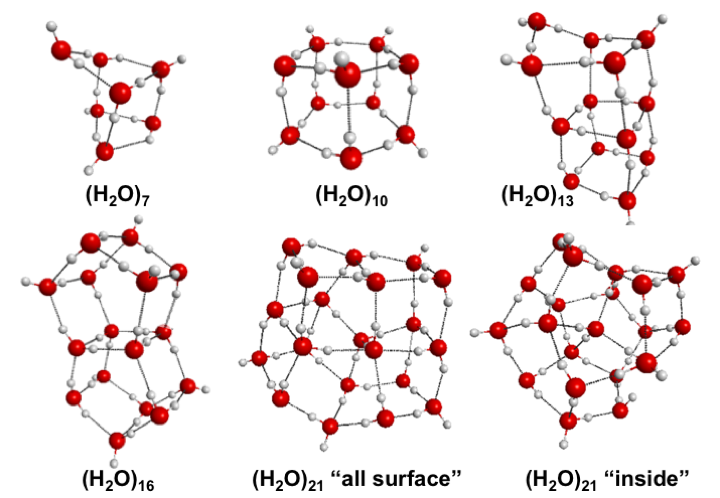
\includegraphics[width=\textwidth]{Figures/Chapter_2/cluster_structures.png}
\end{center}
\label{fig:MBE_I_F1}
\caption[Generating a facing caption page]{Water cluster isomers used in the MBE analysis.}
\end{figure}

\begin{figure}[t]
\uwsinglespace
\begin{center}
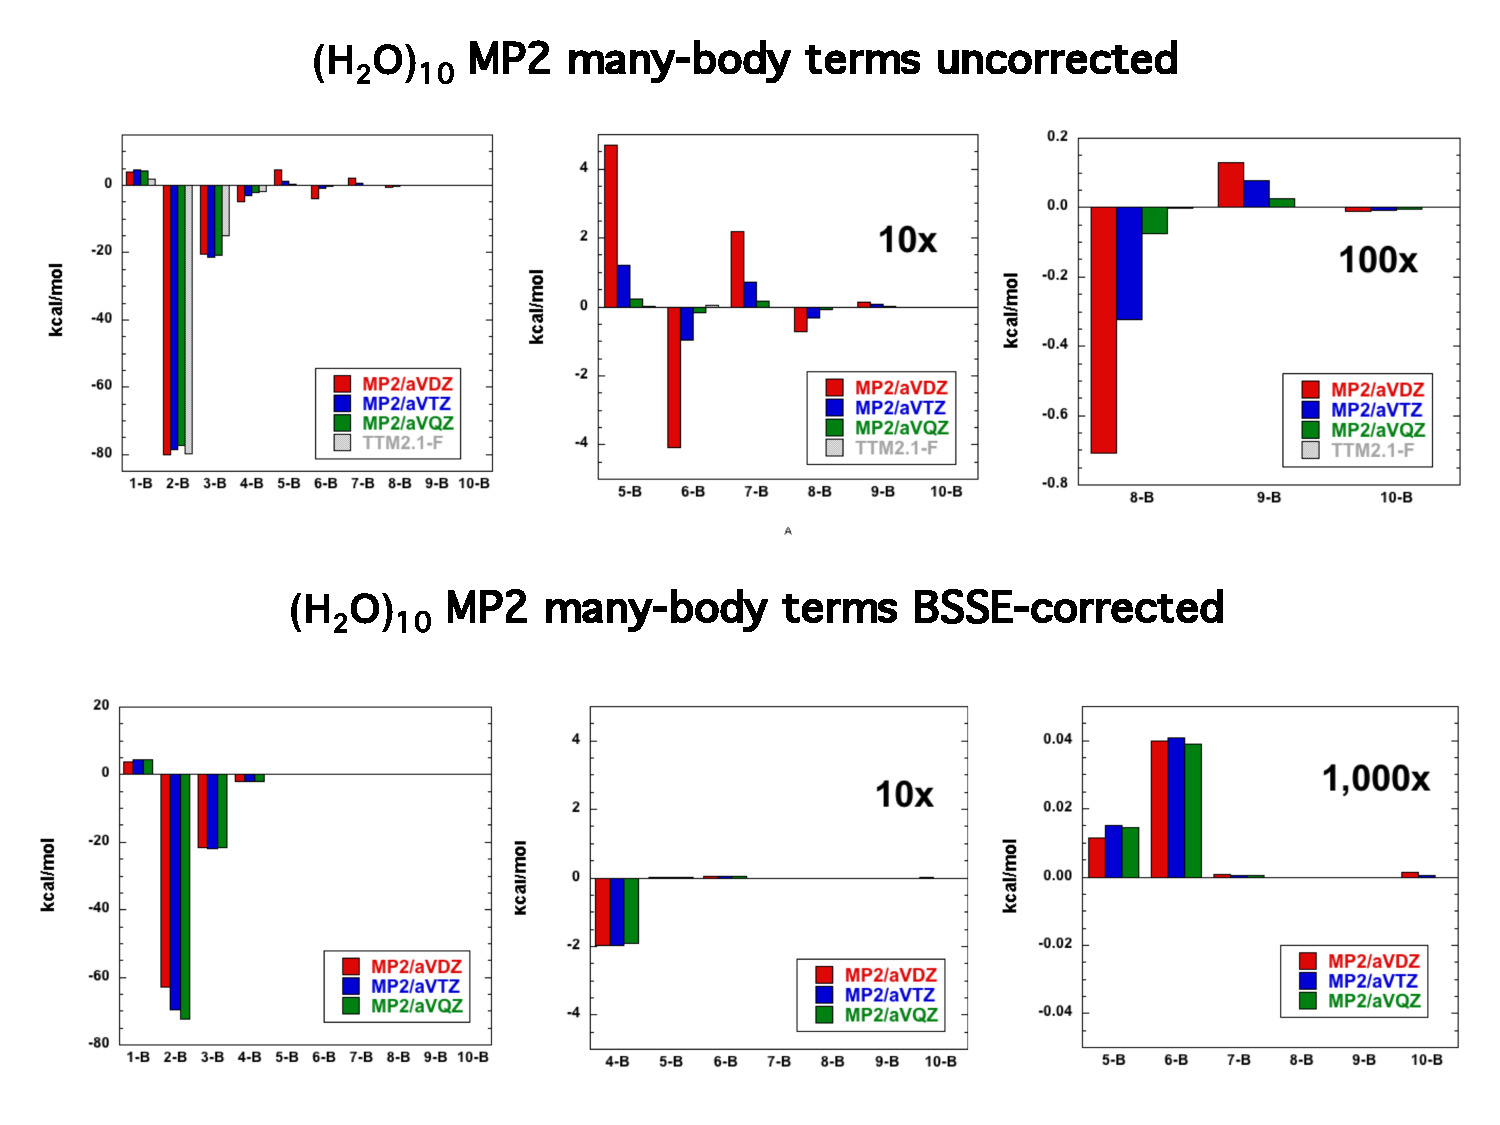
\includegraphics[width=\textwidth]{Figures/Chapter_2/W10_MP2_MB.pdf}
\end{center}
\label{fig:MBE_I_F2}
\caption[temp]{Magnitude of the uncorrected (top) and BSSE-corrected (bottom) 1- through 10-body MBE terms for the \ce{(H2O)_{10}} cluster. Note the magnification (10 – 1000X) of the y-axis in the middle and right panels used to indicate the small magnitude of the higher-order relative to the ones for the 2- and 3-body terms.}
\end{figure}

\begin{figure}[t]
\uwsinglespace
\begin{center}
\begin{minipage}{0.45\textwidth}
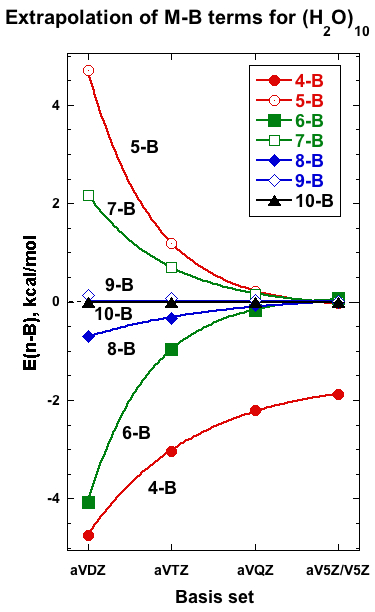
\includegraphics[width=.9\textwidth]{Figures/Chapter_2/MB_extrap_w10_noBSSE.jpg}
\end{minipage}
\begin{minipage}{0.45\textwidth}
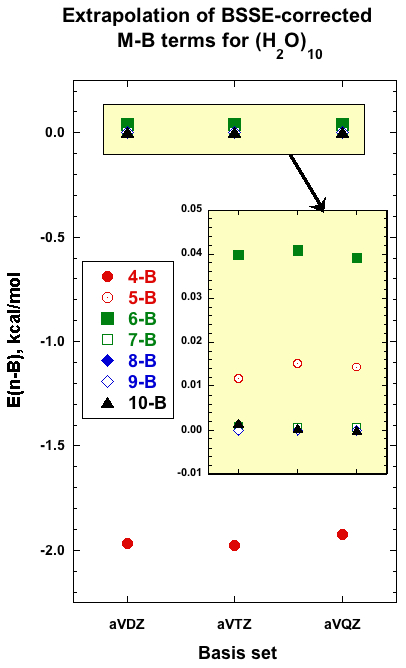
\includegraphics[width=.9\textwidth]{Figures/Chapter_2/MB_extrap_w10_BSSE_all.jpg}
\end{minipage}
\end{center}
\label{fig:MBE_I_F3}
\caption[temp]{Convergence of the uncorrected (left) and BSSE-corrected (right) 4- through 10-body terms in the many-body expansion for \ce{(H2O)_{10}} for the various basis sets. Notice the different y-axis scales.}
\end{figure}

\begin{figure}[t]
\uwsinglespace
\begin{center}
\begin{minipage}{0.45\textwidth}
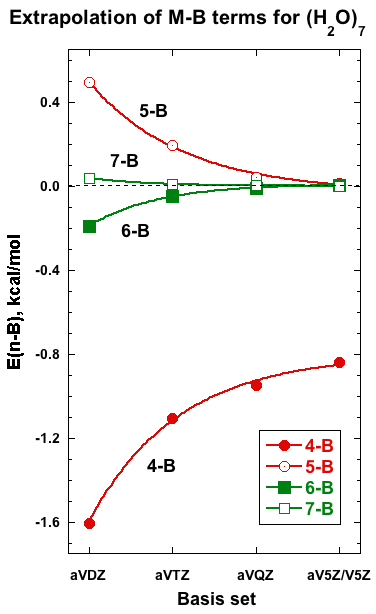
\includegraphics[width=.9\textwidth]{Figures/Chapter_2/MB_extrap_w7_noBSSE.jpg}
\end{minipage}
\begin{minipage}{0.45\textwidth}
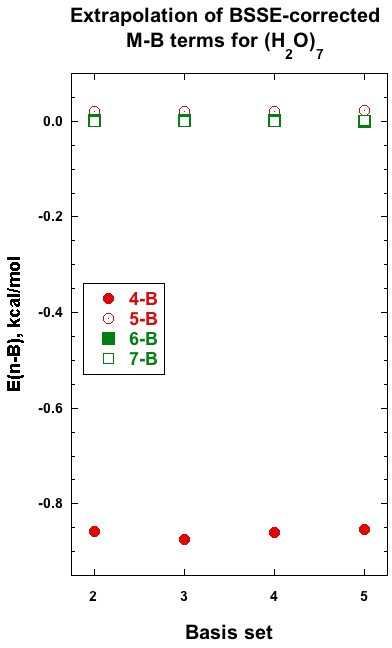
\includegraphics[width=.9\textwidth]{Figures/Chapter_2/MB_extrap_w7_BSSE.jpg}
\end{minipage}
\end{center}
\label{fig:MBE_I_F4}
\caption[temp]{Convergence of the uncorrected (left) and BSSE-corrected (right) 4- through 7-body terms in the many-body expansion for \ce{(H2O)7} for the various basis sets. Notice the different y-axis scales.}
\end{figure}

\begin{figure}[t]
\uwsinglespace
\begin{center}
\begin{minipage}{0.45\textwidth}
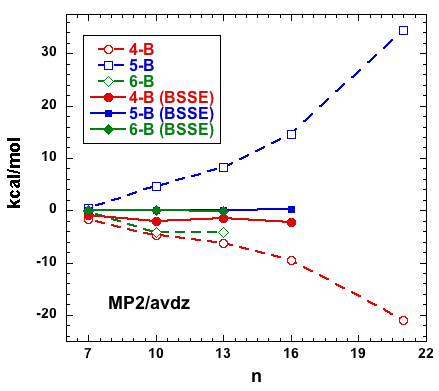
\includegraphics[width=.9\textwidth]{Figures/Chapter_2/4_B_6_B_vs_n.jpg}
\end{minipage}
\begin{minipage}{0.45\textwidth}
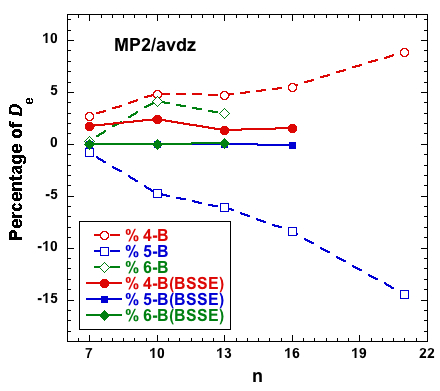
\includegraphics[width=.9\textwidth]{Figures/Chapter_2/4_B_6_B_perc_vs_n.jpg}
\end{minipage}
\end{center}
\label{fig:MBE_I_F5}
\caption[temp]{The absolute magnitudes (left) and percentage contributions (right) of the 4- to 6-body terms to the MP2/AVDZ binding energy for (H2O)n, n = 7, 10, 13, 16 and 21. The uncorrected (dashed lines) and BSSE-corrected results (solid lines) are shown.}
\end{figure}

\begin{figure}[t]
\uwsinglespace
\begin{center}
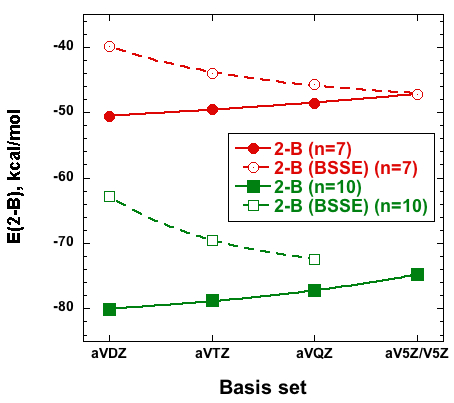
\includegraphics[width=\textwidth]{Figures/Chapter_2/E_2B_7_10.jpg}
\end{center}
\label{fig:MBE_I_F6}
\caption[temp]{Convergence of the uncorrected and BSSE-corrected total 2-body energy for \ce{(H2O)7} and \ce{(H2O)_{10}} with the AVXZ basis sets.}
\end{figure}

\begin{figure}[t]
\uwsinglespace
\begin{center}
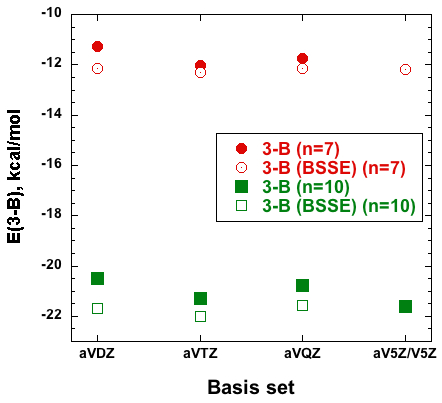
\includegraphics[width=\textwidth]{Figures/Chapter_2/E_3B_7_10.jpg}
\end{center}
\label{fig:MBE_I_F7}
\caption[temp]{Convergence of the uncorrected and BSSE-corrected total 3-body energy for \ce{(H2O)7} and \ce{(H2O)_{10}} with the AVXZ basis sets.}
\end{figure}

\begin{figure}[t]
\uwsinglespace
\begin{center}
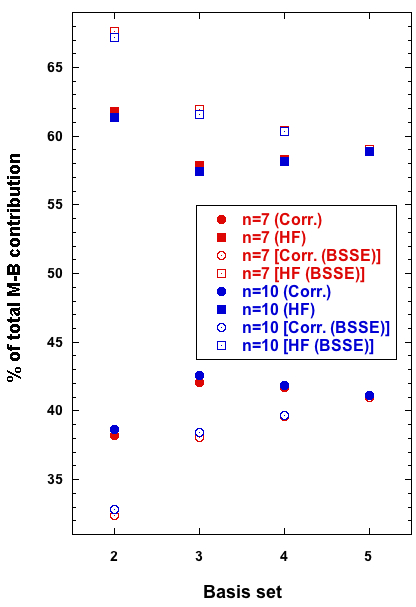
\includegraphics[width=\textwidth]{Figures/Chapter_2/percent_corr_HF_7_10.jpg}
\end{center}
\label{fig:MBE_I_F8}
\caption[temp]{Percentage of the total binding energy from HF and correlation for \ce{(H2O)7} and \ce{(H2O){10}} using the monomer and cluster basis at each of the AVXZ basis sets.}
\end{figure}

\begin{figure}[t]
\uwsinglespace
\begin{center}
\includegraphics[width=\textwidth]{Figures/Chapter_2/2body_bsse_decay_with_basis.tif}
\end{center}
\label{fig:MBE_I_F9}
\caption[temp]{Variation of the BSSE correction for the 2-body terms with the O-O distance between fragments with the different basis sets used in this study. Solid lines represent least mean squares fits of the data to the function $a(1+erf(-bR_{OO}))$ for each basis set.}
\end{figure}

\begin{figure}[t]
\uwsinglespace
\begin{center}
\includegraphics[width=\textwidth]{Figures/Chapter_2/2body_bsse_correlation.tif}
\end{center}
\label{fig:MBE_I_F10}
\caption[temp]{Predicted versus calculated BSSE correction for the individual 2-body terms of the clusters with the different basis sets used in this study.}
\end{figure}

\begin{table}[]
\centering
\begin{tabular}{@{}rrrrrrrrr@{}}
\toprule
     & \multicolumn{4}{c}{Uncorrected}         & \multicolumn{4}{c}{BSSE-corrected}      \\ \midrule
k    & AVDZ    & AVTZ    & AVQZ    & AV5Z/ V5Z & AVDZ    & AVTZ    & AVQZ    & AV5Z/ V5Z \\
\hline
\multicolumn{9}{c}{n = 7}                                                                \\
\hline
1-B  & 2.213   & 2.446   & 2.468   & 2.554     & 2.213   & 2.446   & 2.468   & 2.554     \\
2-B  & -50.578 & -49.459 & -48.626 & -47.160   & -39.894 & -43.958 & -45.712 & -47.165   \\
3-B  & -11.275 & -12.030 & -11.743 & -12.191   & -12.141 & -12.313 & -12.151 & -12.181   \\
4-B  & -1.606  & -1.106  & -0.950  & -0.841    & -0.858  & -0.874  & -0.861  & -0.854    \\
5-B  & 0.493   & 0.194   & 0.043   & 0.013     & 0.021   & 0.021   & 0.020   & 0.023     \\
6-B  & -0.192  & -0.051  & -0.010  & 0.003     & 0.002   & 0.001   & 0.001   & -0.0007   \\
7-B  & 0.037   & 0.008   & 0.002   & -0.0004   & 0.0001  & 0.0001  & 0.0001  & 0.0016    \\
\hline
\multicolumn{9}{c}{n = 10}                                                               \\
\hline
1-B  & 3.952   & 4.509   & 4.449   & 4.595     & 3.952   & 4.509   & 4.449   &           \\
2-B  & -80.165 & -78.707 & -77.249 & -74.796   & -62.762 & -69.504 & -72.387 &           \\
3-B  & -20.475 & -21.285 & -20.790 & -21.625   & -21.691 & -21.989 & -21.582 &           \\
4-B  & -4.742  & -3.028  & -2.202  & -1.878    & -1.968  & -1.978  & -1.923  &           \\
5-B  & 4.698   & 1.200   & 0.219   & -0.038    & 0.012   & 0.015   & 0.014   &           \\
6-B  & -4.081  & -0.964  & -0.179  & 0.071     & 0.040   & 0.041   & 0.039   &           \\
7-B  & 2.175   & 0.708   & 0.1594  & -0.008    & 0.001   & 0.0005  & 0.0005  &           \\
8-B  & -0.707  & -0.324  & -0.0758 & -0.003    & -0.0001 & -0.0001 & -0.0001 &           \\
9-B  & 0.131   & 0.078   & 0.0246  & 0.003     & 0.0000  & 0.0000  & 0.0000  &           \\
10-B & -0.010  & -0.008  & -0.0039 & -0.0006   & 0.0014  & 0.0004  & 0.0000  &           \\ \bottomrule
\end{tabular}
\caption{Magnitudes of the individual terms (kcal/mol) for the clusters \ce{(H2O)n}, n = 7, 10 with the various basis sets. Both the uncorrected and BSSE-corrected values are listed.}
\label{tab:MBE_I_T1}
\end{table}

\begin{table}[]
\centering
\begin{tabular}{@{}rrr@{}}
\toprule
k       & Uncorrected     & BSSE-corrected     \\ \midrule
\multicolumn{3}{c}{n =13}                      \\
\hline
1-B     & 4.527           & 4.527              \\
2-B     & -111.096        & -86.692            \\
3-B     & -26.264         & -28.335            \\
4-B     & -6.352          & -1.499             \\
5-B     & 8.243           & 0.056              \\
6-B     & -4.081          & -0.050             \\
\hline
\multicolumn{3}{c}{n =16}                      \\
\hline
1-B     & 6.456           & 6.456              \\
2-B     & -141.072        & -110.162           \\
3-B     & -35.514         & -37.944            \\
4-B     & -9.463          & -2.179             \\
5-B     & 14.560          & 0.181              \\
\hline
\multicolumn{3}{c}{n =21 					(“all-surface”)} \\
\hline
1-B     & 7.819           &                    \\
2-B     & -191.747        &                    \\
3-B     & -44.152         &                    \\
4-B     & -19.892         &                    \\
5-B     & 39.090          &                    \\
\hline
\multicolumn{3}{c}{n =21 (“inside”)}           \\
\hline
1-B     & 9.585           &                    \\
2-B     & -191.447        &                    \\
3-B     & -47.359         &                    \\
4-B     & -20.976         &                    \\
5-B     & 34.391          &                    \\ \bottomrule
\end{tabular}
\caption{Magnitudes of the individual terms (kcal/mol) for the clusters \ce{(H2O)n}, n = 13, 16, 21 at the MP2/AVDZ level of theory. Both the uncorrected and BSSE-corrected values are listed.}
\label{tab:MBE_I_T2}
\end{table}

\begin{table}[]
\centering
\begin{tabular}{@{}ccccc@{}}
\toprule
Cluster & 1-Body          & 2-Body           & Sum of 3- to 5-Body & Total Correlation \\ \midrule
\ce{(H2O)7}  & -3.73 (15.80)   & -19.77 (83.74)   & -0.105 (0.44)       & -23.609           \\
\ce{(H2O)_{10}} & -6.391 (16.59)  & -31.870 (82.75)  & -0.250 (0.65)       & -38.514           \\
\ce{(H2O)_{13}} & -9.135 (23.99)  & -29.0526 (76.31) & 0.135 (-0.35)       & -38.073           \\
\ce{(H2O)_{16}} & -12.051 (24.80) & -36.205 (74.49)  & -0.344 (0.71)       & -48.600           \\ \bottomrule
\end{tabular}
\caption{Contribution of the correlation energy to the various many-body terms for \ce{(H2O)n}, n = 7, 10, 13, 16. The results are obtained with the largest basis set used for each isomer (see text). The percentage of the total correlation energy is given in parentheses. Energies are in kcal/mol, while parentheses indicate the percentage of the total correlation energy.}
\label{tab:MBE_I_T3}
\end{table}

\begin{table}[]
\centering
\begin{tabular}{@{}lccc@{}}
\toprule
(H2O)3       & \multicolumn{1}{p{3cm}}{\centering MP2/AVQZ//\\MP2/AVQZ} & \multicolumn{1}{p{4cm}}{\centering CCSD(T)/AVQZ//\\MP2/AVQZ} & \multicolumn{1}{p{4cm}}{\centering CCSD(T)/AVQZ//\\CCSD(T)/AVQZ}\\
\hline
\textbf{Total Energy} & \textbf{-15.440}   & \textbf{-15.478}       & \textbf{-15.493}           \\
\hline
1-B          & 0.429              & 0.410                  & 0.346                      \\
2-B          & -13.359            & -13.428                & -13.479                    \\
3-B          & -2.510             & -2.460                 & -2.360           \\ \bottomrule         
\end{tabular}
\caption{The MP2/AVQZ and CCSD(T)/AVQZ 1-, 2-, and 3-body terms for \ce{(H2O)3} at the MP2/AVQZ and CCSD(T)/AVQZ geometries. The notation CCSD(T)/AVQZ//MP2/AVQZ means CCSD(T)/AVQZ energies are calculated the MP2/AVQZ optimized geometry. The relevant monomer reference energies (from left to right), in a.u., are -76.35191864, -76.36358738, and -76.3635876.}
\label{tab:MBE_I_T4}
\end{table}

\begin{table}[]
\centering
\begin{tabular}{@{}ccccc@{}}
\toprule
             & MP2/AVDZ          & CCSD(T)/AVDZ               & MP2/AVTZ          & CCSD(T)/AVTZ \\
             \hline
Total Energy & \textbf{-60.908 / -50.658} & \textbf{-60.841 / -49.900} & \textbf{-59.998 / -54.676} &              \\
\hline
1-B          & 2.213 / 2.213     & 2.075 / 2.075              & 2.446 / 2.446     & 2.372        \\
2-B          & -50.578 / -39.894 & -50.727 / -39.359          & -49.459 / -43.958 & -49.738      \\
3-B          & -11.275 / -12.141 & -10.811 / -11.710          & -12.030 / -12.313 & -11.636      \\
4-B          & -1.606 / -0.858   & -1.758 / -0.937            & -1.106 / -0.874   &              \\
5-B          & 0.493 / 0.021     & 0.553 / 0.027              & 0.194 / 0.021     &              \\
6-B          & -0.192 / 0.002    & -0.212 / 0.002             & -0.51 / 0.001     &              \\
7-B          & 0.037 / 0.000     & 0.040 / 0.000              & 0.008 / 0.000     &             \\ \bottomrule
\end{tabular}
\caption{The MP2/AVXZ and CCSD(T)/AVXZ BSSE-uncorrected and BSSE-corrected interaction energies for \ce{(H2O)7} in the format $E_{uncorr}$ / $E_{corr}$ all carried out at the MP2/AVXZ geometry for X=D, T. The relevant water monomer reference energies (from left to right), in a.u., are -76.26090977, -76.27390289, -76.3289924, and -76.34232562. We do not report the BSSE-corrected numbers for CCSD(T)/AVTZ due to the computational expense.}
\label{tab:MBE_I_T5}
\end{table}

\begin{table}[]
\centering
\begin{tabular}{@{}ccccc@{}}
\toprule
\textbf{Basis set}  & \textbf{a} & \textbf{b} & $\mathbf{\chi}$ & \textbf{R} \\
\hline
aug-cc-pVDZ         & 14.435 & 0.4639 & 0.1342 & 0.9946 \\
aug-cc-pVTZ         & 9.445  & 0.4887 & 0.0386 & 0.9948 \\
aug-cc-pVQZ         & 5.549  & 0.4998 & 0.0131 & 0.9937 \\
aug-cc-pV5Z/cc-pV5Z & 11.211 & 0.6728 & 0.0006 & 0.9931 \\ \bottomrule
\end{tabular}
\caption{Fit of the 2-body BSSE correction via eq. (A.2) for the various basis sets.}
\label{tab:MBE_I_T6}
\end{table}

% ========== Chapter 2
 
\chapter{A Brief \\ Description of \protect\TeX}
 
The \TeX\ formatting program is the creation of
Donald Knuth of Stanford University.
It has been implemented on nearly every general purpose computer and
produces exactly the same copy on all machines.
 
\section{What is it; why is it spelled that way; 
and what do
really long section titles look like in the text and in the
Table of Contents?}
 
\TeX\ is a formatter.  A document's format is controlled
by commands embedded in the text.  
\LaTeX\ is a special version of \TeX---preloaded
with a voluminous set of macros that simplify most
formatting tasks.
 
\TeX\ uses {\it control sequences} to control
the formatting of a document.  These control sequences are usually
words or groups of letters prefaced with the backslash character
({\tt\char'134}).
For example,
Figure \ref{start-2} shows the text that printed the beginning
of this chapter.  Note the control sequence \verb"\chapter" that
instructed \TeX\ to start a new chapter, print the title, and
make an entry in the table of contents.  It is an example
of a macro defined by the \LaTeX\ macro package.
The control sequence \verb"\TeX", which prints the word \TeX,
is a standard macro from the {\it\TeX book}.
The short control sequence \verb"\\" in the title instructed \TeX\ to
break the title line at that point.
This capability is an example of an extension to \LaTeX\
provided by the uwthesis document class.
 
\begin{figure}
\begin{demo}
\uwsinglespace
\\chapter\{A Brief\\\\Description of \\TeX\}

The \\TeX\\ formatting program is the creation of
Donald Knuth of Stanford University.
\end{demo}
\label{start-2}
\caption{The beginning of the Chapter II text}
\end{figure}
 
Most of the time \TeX\ is simply building paragraphs from
text in your source files.  No control sequences are involved.
New paragraphs are indicated by a blank line in the
input file.
Hyphenation is performed automatically.
 
\section{\TeX books}
 
The primary reference for \LaTeX\ is Lamport's second edition
of the \textit{\LaTeX\ User's Guide}\cite{Lbook}.
It is easily read and should be sufficient for thesis formatting.
See also the \textsl{\LaTeX\ Companion}\cite{companion} for descriptions
of many add-on macro packages.

Although unnecessary for thesis writers, the \textsl{\TeX book}
is the primary reference for \TeX sperts worldwide.
 
\section{Mathematics}
 
The thesis class does not expand on \TeX's
or \LaTeX's
comprehensive treatment of mathematical equation printing.%

%
The {\it\TeX book}\cite{book}, {\it \LaTeX\ User's Guide}\cite{Lbook},
and {\it The \LaTeX\ Companion}\cite{companion}
thoroughly cover this topic.
 
 
\section{Languages other than English}
 
Most \LaTeX\ implementations at the University are tailored
for the English language.  However, \LaTeX\ will format many
other languages.  Unfortunately, this author has never been successful in 
learning more than a smattering of anything other than English.
Consult your department or the Tex Users Group.
\smallskip
\begin{center}
{\tt http://tug.org/},
\end{center}
\smallskip
for assistance with non-English formatting.

Unusual characters can be defined via the
font maker \hbox{\mffont METAFONT} (documented by Knuth\cite{Metafont}).
The definitions are not trivial.
Students who attempt to print a thesis with
custom fonts may soon proclaim,
 
% Note.  This is not the ideal way to print Greek
\medskip
\begin{center}
``$\mathaccent"7027\alpha\pi o\kern1pt\theta\alpha\nu\epsilon\hat\iota\nu$
\ $\theta\acute\epsilon\lambda\omega$.''
 
\end{center}
 
% ========== Chapter 3
 
\chapter{The Thesis Unformatted}
 
This chapter describes the uwthesis class (\texttt{uwthesis.cls},
version dated 2014/11/13)
in detail 
and shows how it was used to format the thesis.
A working knowledge of Lamport's \LaTeX\ manual\cite{Lbook} is assumed.
 
\section{The Control File}
 
The source to this sample thesis is a single file
only because ease of distribution was a concern.
You should not do this.  Your task will be much easier if you
break your thesis into several files:  a file for the preliminary pages,
a file for each chapter,  one for the glossary, and one for each
appendix.  Then use a control file to tie them all together.
This way you can edit and format parts of your thesis much more
efficiently.
 
Figure~\ref{control-file} shows a control file that
might have produced this thesis.
It sets the document style, with options and parameters,
and formats the various parts of the thesis---%
but contains no text of its own.
 
 
%  control file caption and figure
%
%
\begin{figure}[p]
 \begin{fullpage}
  \uwsinglespace
  \begin{verbatim}
    % LaTeX thesis control file
 
    \documentclass [11pt, proquest]{uwthesis}[2014/11/13]
 
    \begin{document}
 
    % preliminary pages
    %
    \prelimpages
    \include{prelim}
 
    % text pages
    %
    \textpages
    \include{chap1}
    \include{chap2}
    \include{chap3}
    \include{chap4}
 
    % bibliography
    %
    \bibliographystyle{plain}
    \bibliography{thesis}
 
    % appendices
    %
    \appendix
    \include{appxa}
    \include{appxb}
 
    \include{vita} 
    \end{document}
  \end{verbatim}
  \caption[A thesis control file]%
   {\narrower A thesis control file ({\tt thesis.tex}).
   This file is the input to \LaTeX\ that will produce a
   thesis.  It contains no text, only commands which
   direct the formatting of the thesis.
   }
  \label{control-file}
 \end{fullpage}
\end{figure}
 
The first section, from the \verb"\documentclass" to
the \verb"\begin{document}", defines the document class and options.
This sample thesis specifies the \texttt{proquest} style, which is now
required by the Graduate School and is the default.  
Two other, now dated, other styles are available:  \verb"twoside", which is similar but 
produces a wider binding margin and is more suitable for paper printing; and
\verb"oneside", which is really old fashoned.
This sample also specified a font size
of 11 points. 
Possible font size options are: \verb"10pt", \verb"11pt", and \verb"12pt".
Default is 12 points, which is the preference
of the Graduate School. If you choose a smaller size be sure to
check with the Graduate School for acceptability.  The smaller fonts
can produce very small sub and superscripts.

Include most additional formatting packages with \verb"\usepackage",
as describe by Lamport\cite{Lbook}.  The one exception to this
rule is the \verb"natbib" package.  Include it with the \verb"natbib"
document option.
 
Use the \verb"\includeonly" command to format only a part of your
thesis.  See Lamport\cite[sec. 4.4]{Lbook} for usage and limitations.

 
\section{The Text Pages}
 
A chapter is a major division of the thesis.  Each chapter begins
on a new page and has a Table of Contents entry.
 
\subsection{Chapters, Sections, Subsections, and Appendices}
 
 
Within the chapter title use a \verb"\\" control sequence to separate lines
in the printed title (recall Figure \ref{start-2}.).
The \verb"\\" does not affect the Table of Contents entry.
 
Format appendices just like chapters.
The control sequence \verb"\appendix" instructs \LaTeX\ to
begin using the term `Appendix' rather than `Chapter'.
 
 
Specify sections and subsections of a chapter 
with  \verb"\section" and \verb"\subsection", respectively.
In this thesis chapter and section
titles are written to the table of contents.
Consult Lamport\cite[pg. 176]{Lbook} to see which
subdivisions of the thesis can be written to the table of contents.
The \verb"\\" control sequence is not permitted in section and
subsection titles.
 
 
\subsection{Footnotes}
 
\label{footnotes}
 Footnotes format as described in the \LaTeX\ book.  You can also
 ask for end-of-chapter or end-of-thesis notes.
 The thesis class will automatically set these up if
 you ask for the document class option \texttt{chapternotes}
 or \texttt{endnotes}.  
 
If selected, chapternotes will print automatically.  If you choose
endnotes however you must explicitly indicate when to print the notes 
with the command \verb"\printendnotes".  See the style guide for
suitable endnote placement.  

\subsection{Figures and Tables}
Standard \LaTeX\ figures and tables, see Lamport\cite[sec.~C.9]{Lbook},
normally provide the most convenient means to position the figure.
Full page floats and facing captions are exceptions to this rule.

If you want a figure or table to occupy a full page enclose the
contents in a \texttt{fullpage} environment.  
See figure~\ref{facing-caption}.

\subsubsection{Facing pages}
Facing page captions are an artifact of traditional, dead-tree printing,
where a left-side (even) page faces a right-side (odd) page.

In the \texttt{twoside} style, a facing caption
is full page caption for a full page figure or table
and should face the illustration to which it refers.
You must explicitly format both pages. 
The caption part appears on an even page
(left side) and the figure or table
comes on the following odd page (right side).
Enclose the float contents for the caption 
in a \texttt{leftfullpage} environment,
and enclose the float contents for the figure or table 
in a \texttt{fullpage} environment.
The first page (left side) contains the caption. The second page
(right side) could be left blank.  A picture or graph might be pasted onto
this space. See figure~\ref{facing-caption}.


\begin{figure}[t]
\uwsinglespace
\begin{verbatim}
     \begin{figure}[p]% the left side caption
       \begin{leftfullpage}
         \caption{ . . . }
       \end{leftfullpage}
     \end{figure}
     \begin{figure}[p]% the right side space
       \begin{fullpage}
          . . .
          ( note.. no caption here )
       \end{fullpage}
     \end{figure}
\end{verbatim}
\caption[Generating a facing caption page]{This text would create a
  double page figure in the two-side styles. }
\label{facing-caption}
\end{figure}
 
You can use these commands with the \texttt{proquest} style, but they have little
effect on online viewing.
 
 
\subsection{Horizontal Figures and Tables}
Figures and tables may be formatted horizontally
(a.k.a.\ landscape) as long as their captions appear
horizontal also.  \LaTeX\ will format landscape material for you.

Include the \texttt{rotating} package 
\begin{demo}
\\usepackage[figuresright]\{rotating\}
\end{demo}
and read the documentation that comes with the package. 

Figure~\ref{sideways} is an example of how a landscape
table might be formatted. 

\begin{figure}[t]
\uwsinglespace
\begin{verbatim}
     \begin{sidewaystable}
         ...
         \caption{ . . . }
     \end{sidewaystable}
\end{verbatim}
\caption[Generating a landscape table]{This text would create a
  landscape table with caption.}
\label{sideways}
\end{figure}
 


\subsection{Figure and Table Captions}
Most captions are formatted with the \verb"\caption" macro as described 
by Lamport\cite[sec. C.9]{Lbook}. 
The uwthesis class extends this macro to allow
continued figures and tables, and to provide multiple figures and
tables with the same number, e.g., 3.1a, 3.1b, etc.
 
To format the caption for the first part of
a figure or table that cannot fit
onto a single page use the standard form:
\begin{demo}
\\caption[\textit{toc}]\{\textit{text}\}
\end{demo}
To format the caption for the subsequent parts of 
the figure or table 
use this caption:
\begin{demo}
\\caption(-)\{(continued)\}
\end{demo}
It will keep the same number and the text of the caption will be 
{\em(continued)}.

To format the caption for the first part of
a multi-part figure or table
use the format:
\begin{demo}
\\caption(a)[\textit{toc}]\{\textit{text}\}
\end{demo}
The figure or table will be lettered (with `a') as well as numbered.
To format the caption for the subsequent parts of 
the multi-part figure or table
use the format:
\begin{demo}
\\caption(\textit{x})\{\textit{text}\}
\end{demo}
where {\em x} is {\tt b}, {\tt c}, \ldots.
The parts will be lettered (with `b', `c', \ldots).

If you want a normal caption, but don't want a ToC entry:
\begin{demo}
\\caption()\{\textit{text}\}
\end{demo}
Note that the caption number will increment.  You would normally use this 
only to leave an entire chapter's captions off the ToC.


\subsection{Line spacing}

Normally line spacing will come out like it should. However, the 
ProQuest style allows single spacing in certain situations:
figure content, some lists, and etc.
Use \verb"\uwsinglespace" to switch to single spacing within
a \verb"\begin{}" and \verb"\end{}" block.
The code examples in this document does this. 

\section{The Preliminary Pages}
 
These are easy to format only because they are relatively invariant
among theses.  Therefore the difficulties have already been encountered
and overcome by \LaTeX\ and the thesis document classes.

Start with the definitions that describe your thesis.
This sample thesis was printed with the parameters:

\begin{demo}
\\Title\{The Suitability of the \\LaTeX\\ Text Formatter\\\\
   for Thesis Preparation by Technical and\\\\
   Non-technical Degree Candidates\}
\\Author\{Jim Fox\}
\\Program\{IT Infrastructure\}
\\Year\{2012\}

\\Chair\{Name of Chairperson\}\{title\}\{Chair's department\}
\\Signature\{First committee member\}
\\Signature\{Next committee member\}
\\Signature\{etc\}

\end{demo}
 
Use two or more \verb"\Chair" lines if you have co-chairs.
 
\subsection{Copyright page}
Print the copyright page with \verb"\copyrightpage".

\subsection{Title page}
Print the title page with \verb"\titlepage".
The title page of this thesis was printed with%
 
\begin{demo}
\\titlepage
\end{demo}
 
You may change default text on the title page with these
macros.  You will have to redefine \verb"\Degreetext", for instance,
if you're writing a Master's thesis instead of a dissertation.\footnote{If you use these they can
be included with the other information before \\copyrightpage".}

\begin{list}{}{\itemindent\parindent\itemsep0pt
   \def\makelabel#1{\texttt{\char`\\#1}\hfill}\uwsinglespace}
\item[Degree\char`\{{\it degree name}\char`\}]
   defaults to ``Doctor of Philosophy''
\item[School\char`\{{\it school name}\char`\}] defaults to
``University of Washington''
\item[Degreetext\char`\{{\it degree text}\char`\}] defaults to
``A dissertation submitted \ldots''
\item[textofCommittee\char`\{{\it committee label}\char`\}] defaults to
``Reading Committee:''
\item[textofChair\char`\{{\it chair label}\char`\}] defaults to
``Chair of the Supervisory Committee:''
\end{list}

These definitions must appear \underline{before} the \verb"\titlepage" command.

 
\subsection{Abstract}
Print the
abstract with \verb"\abstract".
It has one argument, which is the text of the abstract.
All the names have already been defined.
The abstract of this thesis was printed with
 
\begin{demo}
\\abstract\{This sample . . . `real' dissertation.\}
\end{demo}
 
 
\subsection{Tables of contents}
Use the standard \LaTeX\ commands to format these items.
 
 
\subsection{Acknowledgments}
Use the \verb"\acknowledgments" macro to format the acknowledgments page.
It has one argument, which is the text of the acknowledgment.
The acknowledgments of this thesis was printed with
 
\begin{demo}
\\acknowledgments\{The author wishes . . . \{\\it il miglior fabbro\}.\\par\}\}
\end{demo}
 
 
\subsection{Dedication}
Use the \verb"\dedication" macro to format the dedication page.
It has one argument, which is the text of the dedication.
 
\subsection{Vita}
Use the \verb"\vita" macro to format the curriculum vitae.
It has one argument, which chronicles your life's accomplishments.

Note that the Vita is not really a preliminary page.
It appears at the end of your thesis, just after the appendices.
 
 
%%  
%% \section{Customization of the Macros}
%%  
%% Simple customization, including 
%% alteration of default parameters,  changes to dimensions,
%% paragraph indentation, and margins, are not too difficult.
%% You have the choice of modifying the class file ({\tt uwthesis.cls})
%% or loading
%% one or more personal style files to customize your thesis.
%% The latter is usually most convenient, since you do not need
%% to edit the large and complicated class file.
%% 
 


% ========== Chapter 4
 
\chapter{Running \LaTeX\\
  ({\it and printing if you must})}
 
 
From a given source \TeX\ will produce exactly the same document
on all computers and, if needed, on all printers.  {\it Exactly the same}
means that the various spacings, line and page breaks, and
even hyphenations will occur at the same places.

How you edit your text files and run \LaTeX\ varies
from system to system and depends on your personal preference.

\section{Running}

The author is woefully out of his depth where 
\TeX\ on Windows is concerned.  Google would be his resource.
On a linux system he types

\begin{demo}
\$\ pdflatex uwthesis
\end{demo}

and it generally works.

 
\section{Printing}
 
All implementations of \TeX\ provide the option of {\bf pdf} output,
which is all the Graduate School requires.  Even if you intend to
print a copy of your thesis create a 
{\tt pdf}.  It will print most anywhere.

\printendnotes

%
% ==========   Bibliography
%
%\nocite{*}   % include everything in the uwthesis.bib file
\printbibliography
%
% ==========   Appendices
%
\appendix
\raggedbottom\sloppy
 
% ========== Appendix A
 
\chapter{Where to find the files}
 
The uwthesis class file, {\tt uwthesis.cls}, contains the parameter settings,
macro definitions, and other \TeX nical commands which
allow \LaTeX\ to format a thesis.  
The source to
the document you are reading, {\tt uwthesis.tex},
contains many formatting examples
which you may find useful.
The bibliography database, {\tt uwthesis.bib}, contains instructions
to BibTeX to create and format the bibliography.
You can find the latest of these files on:

\begin{itemize}
\item My page.
\begin{description}
\item[] \verb%https://staff.washington.edu/fox/tex/thesis.shtml%
\end{description}

\item CTAN
\begin{description}
\item[]  \verb%http://tug.ctan.org/tex-archive/macros/latex/contrib/uwthesis/%
\item[]  (not always as up-to-date as my site)
\end{description}

\end{itemize}

\vita{Jim Fox is a Software Engineer with IT Infrastructure Division at the University of Washington.
His duties do not include maintaining this package.  That is rather
an avocation which he enjoys as time and circumstance allow.

He welcomes your comments to {\tt fox@uw.edu}.
}


\end{document}
